\documentclass{standalone}
\usepackage{tikz}

\title{Rocket}
\begin{document}
	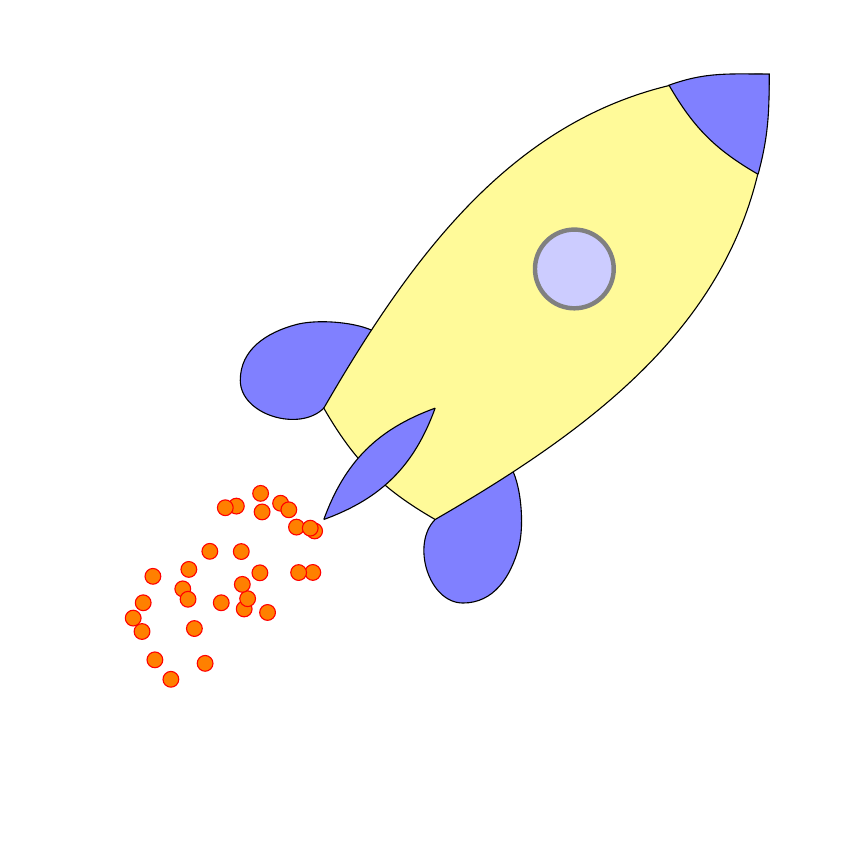
\begin{tikzpicture}
		\draw[help lines, color=white] (-8,-8) grid (2,2);
		\begin{scope}[rotate=45]
			%flaps
			\coordinate (P) at (-5,-1);
			\draw[fill=blue!50!white] (-5,1) to[out=180,in=225] (-5.5,2) to[out=45,in=150] (-4.5,2) to[out=330,in=0] (-4,1) -- (-5,1);
			\begin{scope}[rotate around={180:(P)},shift={(-10cm,-2cm)},yscale=1,xscale=-1]
				\draw[fill=blue!50!white] (-5,1) to[out=180,in=225] (-5.5,2) to[out=45,in=150] (-4.5,2) to[out=330,in=0] (-4,1) -- (-5,1);
			\end{scope}
			%rocket
			\draw[fill=yellow!40!white] (-5,-1) to[out=105,in=255] (-5,1) to[out=15,in=135] (2,0) to[out=225,in=345] (-5,-1);
			%peak
			\draw[fill=blue!50!white] (1,-0.8) to[out=105,in=255] (1,0.8) to[out=335,in=135] (2,0) to[out=225,in=30] (1,-0.8);
			%central flap
			\draw[fill=blue!50!white] (-6,0) to[out=335,in=205] (-4,0) (-6,0) to[out=25,in=155] (-4,0);
			%porthole
			\draw[color=gray,ultra thick,fill=white!80!blue] (-1.5,0) circle (0.5cm);
			%fuel
			\foreach \i in {1,2,...,30}{
				\pgfmathsetmacro{\x}{(rand*0.2 + 1)*-7 - 0.5}
				\pgfmathsetmacro{\y}{(rand*0.5 + 1)*1.5-1.2}
				\pgfmathsetmacro{\opacVal}{rand*0.5+1}
				\draw[color=red, fill=red!50!yellow] (\x,\y) circle (0.1cm);
			}
		\end{scope}
	\end{tikzpicture}
\end{document}
